% Options for packages loaded elsewhere
\PassOptionsToPackage{unicode}{hyperref}
\PassOptionsToPackage{hyphens}{url}
%
\documentclass[11pt]{ctexart}
\usepackage[vmargin=1.5cm, hmargin=2.5cm]{geometry}

\usepackage{amssymb,amsmath}
\usepackage{xcolor}
\usepackage{hyperref}
\hypersetup{hidelinks}
\urlstyle{same} % disable monospaced font for URLs
\usepackage{graphicx}

%%%%%%%%%% SET CJK FONT
\usepackage{fourier}
\setCJKmainfont[ItalicFont=Adobe Kaiti Std, SmallCapsFont=*]{Noto Sans CJK SC}
\setCJKsansfont{Noto Sans CJK SC}
\setCJKmonofont{Noto Sans Mono CJK SC}
%%%%%%%%%%%%%%%%%%%%%%%%%%

%%%%%%%%%%%%%%%%%%%%%%%%%%%%%%%%%%%%%
\usepackage{fancyhdr}
\pagestyle{fancy} 
\fancyhead[L]{\textit{《宏观经济学》}}
\fancyhead[C]{\texttt{第} \thepage \textit{页}}
\fancyhead[R]{\textit{数字经济专业}}
\fancyfoot[L]{\textit{湖南大学课程}}
\fancyfoot[R]{\thepage}
\fancyfoot[C]{\textit{授课教师:雷浩然}}
%%%%%%%%%%%%%%%%%%%%%%%%%%%%%%%%%%%%%

\author{}
\date{}

\begin{document}
\begin{center}
  \subsection*{IS-LM: 产品市场和货币市场的短期均衡}
\end{center}

\paragraph{产品市场与 IS 曲线}
\begin{itemize}
\item
  凯恩斯交叉模型中假设:计划投资水平 $\bar{I}$ 外生固定
\item
  实际生活中:投资需求取决于融资成本,即(借贷)利率 $r$

  \begin{itemize}
  \item
    投资函数:$I = I(r)$. 这是减函数,对应的曲线向下倾斜。
  \item
    图 \ref{fig:is} 的三个子图的含义:(a)利率提高导致计划投资下降
    (b)投资支出下降导致计划支出下降,从而使均衡产出下降
    (c)综合前两者,利率提高导致均衡产出下降
  \end{itemize}
\end{itemize}

\begin{figure}[htbp]
\centering
\includegraphics[width=0.8\textwidth]{~/Downloads/is-curve.jpeg}
\caption{产品市场均衡: IS 曲线}
\label{fig:is}
\end{figure}

IS 曲线方程: 
\begin{equation*}
Y = C(Y) + I(r) + G. 
\tag{IS}  
\end{equation*}

方程(IS)包含两个内生变量 $Y$和 $r$, 我们还需要考虑货币市场的均衡才能确定均衡时的总产出$Y$和利率$r$.

IS = ``\textbf{I}nvestment and \textbf{S}avings", LM = ``\textbf{L}iquidity and \textbf{M}oney supply''

\paragraph{流动性偏好 (Liquidity preference)}
\begin{itemize}
\item
  IS 曲线中利率是外生给定的, 我们无法得知利率是如何决定的.
\item
  凯恩斯在《通论》一书中提出``流动性偏好''理论.
\item
  之所以叫``流动性偏好'',是因为这个理论分析的是货币市场,而``流动性''是人们愿意``持有货币''而非资产的原因. 这里的资产包括实体资产和除了货币以外的金融资产.
\end{itemize}

\paragraph{实际货币余额供给}

\begin{itemize}
\item
  假设货币供给为 M, 价格水平为 P, 则实际货币余额供给为 $M/P$.
\item
  一般认为, 实际货币余额的\textbf{供给}是外生给定的: $(M/P)^s = \bar{M}/ \bar{P}$

  \begin{itemize}
  \item
    这是个很强的假设, 它甚至都不取决于利率
  \item
    假设的理由: 名义货币供给 $\bar{M}$ 由央行决定, 价格水平 $\bar{P}$ 在短期不变
  \end{itemize}
\end{itemize}

\paragraph{实际货币余额需求 (流动性偏好理论)}

\begin{itemize}
\item
  实际货币余额需求由利率和产出决定:$(M/P)^d = L(Y, r)$
\item
  利率是持有货币的机会成本. 这里的利率应该理解为回报率, 比如购买债券的利率.
  
  张三月入一万, 他考虑将财富在两种资产(货币和债券)上进行分配:

  \begin{itemize}
  \item
    货币流动性高, 可直接用于交易; 但货币不能生息.
  \item
    债券的收益率为 $r$, 但流动性差, 一般不能直接用于购买商品.
  \item
    利率上升时, 人们愿意牺牲更多的流动性 (即持有更少货币), 以换取高投资回报.
  \end{itemize}
\end{itemize}

\begin{center}
\begin{figure}[htbp]
\centering
\includegraphics[width = 0.6\textwidth]{~/Downloads/money-demand.jpeg}
\caption{\centering 均衡利率 $r$. 均衡利率由实际货币余额的供给和需求决定, 这个图固定了收入 $Y$, 只考虑 $r$ 对实际货币余额需求的影响.}
\end{figure}  
\end{center}

\paragraph{LM 曲线}

收入 $Y$ 对实际货币余额需求 $L(Y,r)$ 的影响:

\begin{itemize}
\item
  收入高时, 日常开支也高, 人们需要持有更多的货币以便交易.
\item
  $(M/P)^d = L(Y, r)$: 与 $Y$ 正相关,与 $r$ 负相关
\end{itemize}

推导 LM 曲线:

\begin{itemize}
\item
  收入上升导致实际货币余额的需求上升,从而使利率上升: 图3a
\item
  因此, 货币市场的均衡利率与收入 $Y$ 正相关: 图3b
\end{itemize}

\begin{figure}[htbp]
\centering
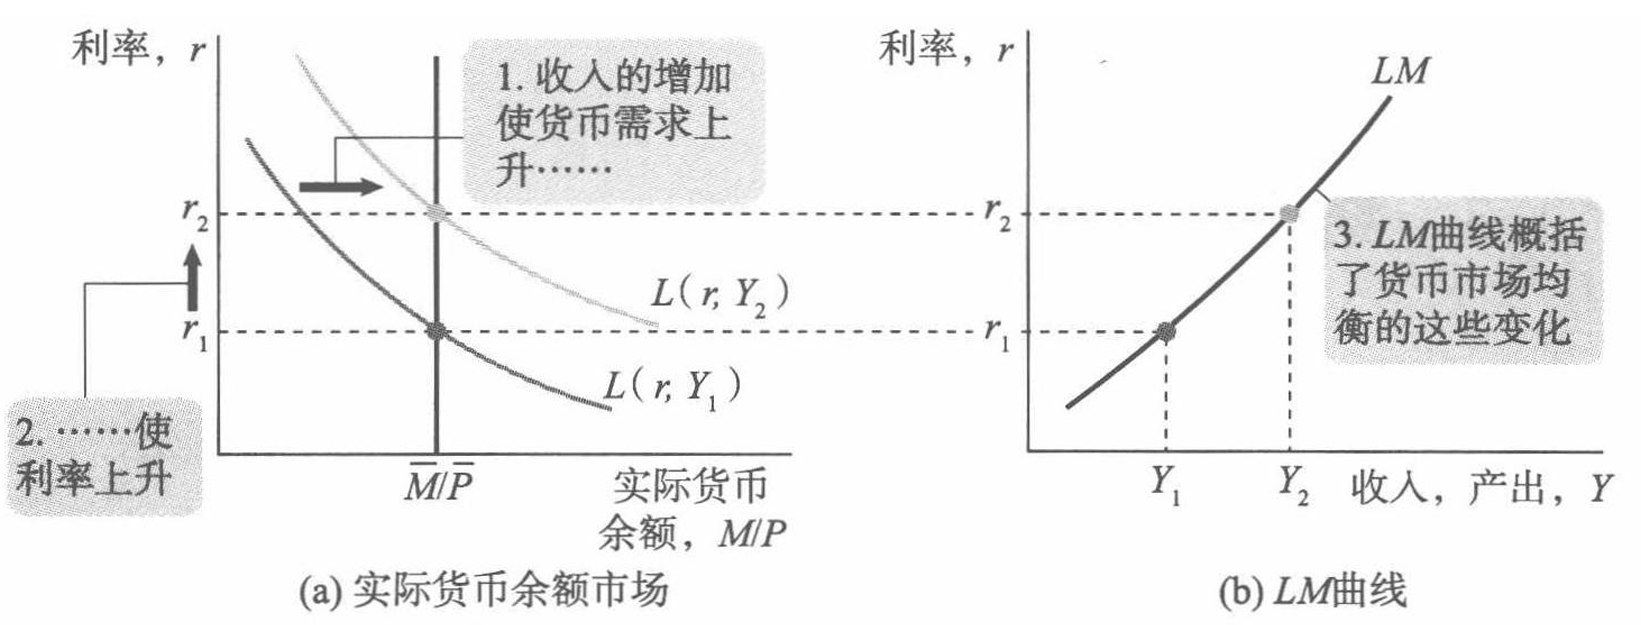
\includegraphics[width=0.9\textwidth]{~/Dropbox/hnu-macro-2021/IMG_0717.jpg}
\caption{由流动性偏好理论推导 LM 曲线}
\end{figure}

\paragraph{IS-LM 模型}

\[Y = C(Y-T) + I(r) + G \tag{IS}\]
\[{\overline{M} / \overline{P}} = L(r,Y) \tag{LM}\]
\begin{itemize}
\item
  IS 曲线表示产品市场的均衡, 均衡条件是``投资等于储蓄''. 
\item
  LM 曲线表示货币市场的均衡, 均衡条件是``实际货币余额的供给等于需求''.
\item
  模型的内生变量: $Y$, $r$; 外生变量包括税收 $T$, 政府购买 $G$, 名义货币供给 $\bar{M}$, 价格 $\bar{P}$.  
\end{itemize}

\begin{figure}[htbp]
\centering
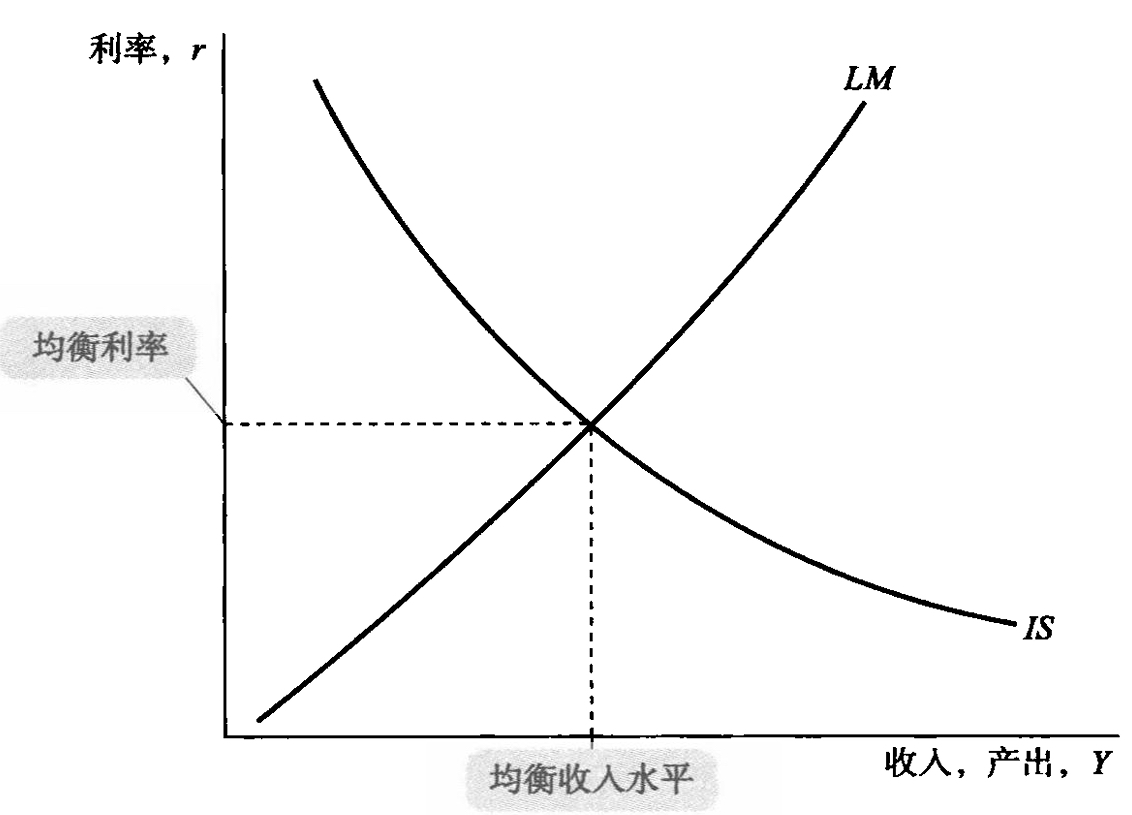
\includegraphics[width=0.5\textwidth]{/Users/lhr45678/Dropbox/hnu-macro-2021/IMG_0718.jpg}
\caption{IS-LM 曲线}
\label{fig:is-lm2}
\end{figure}

\paragraph{总结}

\begin{enumerate}
\item
  IS 曲线: 理论基础是凯恩斯交叉模型. 曲线向下倾斜, 因为更高的利率会降低投资, 进而降低总收入.
\item
  流动性偏好理论: 人们愿意持有货币, 是因为货币可以提供流动性. 实际货币余额的(流动性)需求 $L(Y,r)$ 和$Y$正相关, 和 $r$负相关.
\item
  LM 曲线: 理论基础是流动性偏好. 曲线向上倾斜, 因为更高的收入提高了实际货币余额需求, 进而提高了利率.
\item
  IS 曲线表示满足产品市场均衡的利率与收入, LM
  曲线表示满足货币市场均衡的利率与收入, 其交点表示同时满足这两个市场均衡的利率与收入, 见图 \ref{fig:is-lm2}. 
\end{enumerate}

学习了 IS-LM 模型, 同学们就可以像宏观经济学家一样,
自如地分析\textbf{货币政策和财政政策}的短期经济影响.
这部分内容我们留到之后再专门讨论.

%此外, IS-LM 模型也是下一章推导总需求曲线的理论基础.
%这一部分的理论脉络见下图,
%我们的终极目标是一个可用于描绘\textbf{短期内经济波动}的模型.
%
%\begin{figure}[h]
%\centering
%\includegraphics[width=0.9\textwidth]{~/Downloads/IMG_0719.jpg}
%\end{figure}

\paragraph{练习}
考虑三部门经济, 已知 $C=800+0.63Y$, $I = 7500-20000r$,
$L=0.1625Y-10000r$, $G=7500$, 名义货币供给 $\bar{M} = 6000$, 价格水平 $\bar{P} = 1$.
(1) 推导IS曲线.
(2) 推导LM曲线.
(3) 计算均衡时的利率和投资水平.
(4) 当政府购买上升到 $8500$ 时, 计算私人投资的变化.
\hfill{(\textit{教材106页, Q7})}

\end{document}